\chapter{Application Layer}
The application layer is the fundamental reason why the Internet has been built: the goal is to make something useful and practical with networks, not just route packets.

A \keyword{network application} consists of multiple programs that run on different end-points that communicate over the network. 

\section{Architectures}
There are two main network application architectures:
\begin{itemize}
    \item \emph{client-server}: there is one host, the server, that provides services to the other hosts, the clients. Clients do not communicate with each other. The server has a fixed, well-known address (hostname or IP address) so that a client can contact it by sending a request.
    \item \emph{peer-to-peer} (P2P): all hosts are peers that communicate directly with each other to both provide and request services. However, pure P2P architectures are rare: most applications incorporate a central server to facilitate communication between peers by maintaining a list of their addresses.
\end{itemize}

\section{Processes, Sockets and Ports}
What we called programs are actually processes\footnote{The program is the source code, while the process is the program running inside the operating system.}. 
On a host, there are typically several running processes, so we need a way to make the messages arrive to the right process.

A program of a network application -- hence a program at the Application layer -- makes use of the Transport layer via a \keyword{socket}, that is an abstraction provided by the OS.
It is called socket because you can \q{plug} your message into it to send it to the network (layer) as you would do to provide electricity to a device with an electrical socket.

Coming back to processes and their communication, suppose the host A wants to send a message to the host B. 
A knows B's address -- in some way that we will see -- but does not know which process of A must receive the message.
To choose the right process, B must also know the correct \keyword{port}. 
If an address identifies a \q{building}, a port identifies a \q{mailbox}.
Ports are identified with integer numbers ranging from 0 to 65,535.
Behind the right port, the right process will be hearing for the message.

A postman has to deliver a mail (message) to Jim (the process). The postman has to know Jim's address (IP address), and also Jim's mailbox (port). Jim (the process) will go to his mailbox (port) and pick up his mail (message).

It is convenient to use ports and not process identifiers (PIDs) because, continuing with the postman simile, if another person relocates to Jim's apartment, the port remains the same, with the same number.
The actual main reason why we use ports and not PIDs is that port numbers are standardized\footnote{Port numbers are standardized by IANA and the official, up-to-date list of standard ports are available at the following URL: \url{https://www.iana.org/assignments/service-names-port-numbers/service-names-port-numbers.xhtml}}: notorious processes -- such as an email client or a database -- are always \emph{bound} to the same, standard port. 

\subsection{Choosing the right Transport Protocol for an Application}
The transport layer offers protocols that provide a specific \keyword{Quality of Service} (QoS). Qualities are reliability, throughput, timing, encryption, congestion/flow control.
The network application designer can choose among a set of transport protocols based on the qualities it provides.

\subsubsection{Reliability}
A communication is said reliable when it satisfies all the following three properties:
\begin{enumerate}
    \item \emph{Non corrupted messages}. None of the transmitted bits are corrupted.
    \item \emph{Non lost messages}. None of the transmitted bits are lost or duplicated.
    \item \emph{Correct order of messages}. All of the transmitted bits must arrive in the exact same order in which they were sent.
\end{enumerate}

The assumption is that the lower levels are unreliable. This is generally true (TCP is an exception).

\section{Domain Name System}
People prefer to connect to online resources using hostnames, while for machines IP addresses are more convenient. The \keyword{Domain Name System} (DNS) is a translation protocol that allows to find an IP address given a hostname. 
What the DNS does is the Internet for most people.

A DNS system is implemented with a client-server architecture: each end-point has a DNS client that queries the DNS server with the hostname.
The DNS server perform a look up and find the associated IP. This look-up table may be dynamic: querying for the same hostname at different times may yield different IP addresses.

Since there's a bunch of hostnames and IP addresses in the world, a single, big look-up table would be really slow and would be a single point of failure for the entire Internet.
In fact, the DNS server system was designed with a hierarchical structure, as shown in Figure~\ref{fig:dns_tree}.

\begin{figure}[htbp]
    \centering
    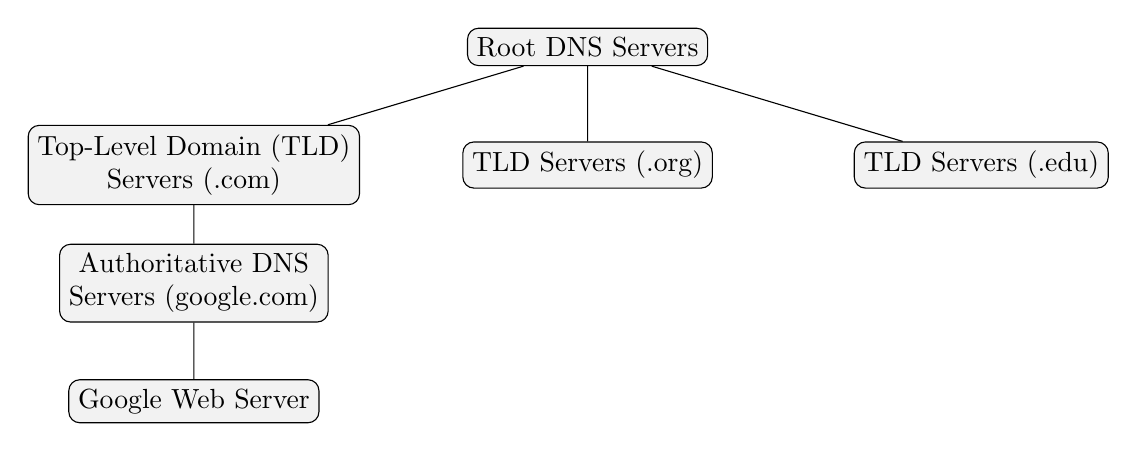
\begin{tikzpicture}[
        level distance=1.5cm,
        sibling distance=5cm,
        every node/.style={shape=rectangle, draw, align=center, rounded corners, fill=gray!10}
    ]
    \node {Root DNS Servers}
        child {node {Top-Level Domain (TLD)\\ Servers (.com)}
            child {node {Authoritative DNS\\ Servers (google.com)}
                child {node {Google Web Server}}
            }
        }
        child {node {TLD Servers (.org)}}
        child {node {TLD Servers (.edu)}};
    \end{tikzpicture}
    \caption{The hierarchical structure of the Domain Name System infrastructure.}
    \label{fig:dns_tree}
\end{figure}

Here’s what happens:
\begin{enumerate}
    \item You request gmail.com.
    \item The root DNS server tells the user's DNS to contact a top-level DNS server for .com.
    \item The top-level DNS server tells the user's DNS to contact an authoritative DNS server for Google.
    \item The authoritative DNS server tells the user's DNS the IP address of the server.
\end{enumerate}

If the domain resolving required all these steps, it would be slower than the implementation we are used to.
In fact, to speed up the process, we make use of \keyword{DNS resolvers}, that technical people simply call DNSs.
DNSs are identified by an IP address, but they usually come with a primary and a secondary address.
For example, Google provides a DNS resolver with \texttt{8.8.8.8} and \texttt{8.8.4.4} as primary and secondary addresses respectively.

\section{Peer-to-peer File Sharing: BitTorrent}
BitTorrent is the most common peer-to-peer (\keyword{p2p}) protocol for file sharing. It is based on the concept of \keyword{torrent}, that is a group of peers participating to the distribution of a file. 
Files are splitted into fixed-sized \keyword{chunks} so that a complete download is made of several sub-downloads.
In this way, a peer can begin to share its chunks even before they have the entire file.
This maximizes the file distribution, which is crucial for the torrent performance: if more peers have the file, a new peer can download that file faster.

As we said before, pure p2p applications are rare and BitTorrent is not one of these.
In fact, each torrent has a \keyword{tracker}, a server that keeps track of the peers participating to the torrent. 
When a peer joins a torrent:
\begin{enumerate}
    \item The tracker registers it.
    \item The tracker sends the IP address of the new peer to a random subset of peers in the torrent.
    \item The new peer can now establish TCP connections with all of its peers (called neighbors).
    \item The peer requests chunks following the \emph{rarest-first} principle: the least distributed chunks are first requested to balance the chunk distribution across the torrent. Having rare chunks is a risk for the complete file integrity: if such chunks disappear, the entire file cannot be downloaded anymore.
    \item The peer uploads its chunks following two principles:
        \begin{itemize}
            \item The peer prioritizes the four best neighbors. Neighbors can be updated periodically -- usually ten seconds -- to find better ones;
            \item Periodically -- usually thirty seconds -- the peer picks a random peer from the torrent and sends its chunks to it. If the exchange is successful, the two peers add each other to their \emph{best list}. This allows peers to select the most compatible neighbors over time.
        \end{itemize}
\end{enumerate}

\section{The World Wide Web and HTTP}
The \emph{World Wide Web} (\keyword{WWW}) is a collection of informations that can be accessed over the Internet via, mostly, the \emph{HyperText Transfer Protocol} (\keyword{HTTP}).

HTTP-based communication is typically client-server: a client program sends a HTTP \emph{request} to the server, that receives the request, executes its related operations and sends a HTTP \emph{response} back to the client.

The HTTP protocol defines the structure of the messages and the way the client and the server exchange such messages -- as all protocols do.

Every resource on the WWW is identified by a Uniform Resource Locator (URL). According to RFC 3986~\cite{rfc3986}, a URL is a string conforming to the following general format:

\begin{example}{URL Syntax}
\texttt{scheme:[//[userinfo@]host[:port]]path[?query][\#fragment]}
\end{example}

The components are defined as follows:
\begin{itemize}
    \item \emph{scheme}: Identifies the protocol used to access the resource (e.g., \texttt{http}, \texttt{https}).
    \item \emph{userinfo} (optional): Contains authentication information, though this is heavily deprecated for security reasons.
    \item \emph{host}: The domain name or IP address of the server hosting the resource.
    \item \emph{port} (optional): The TCP port number on which the server is listening. If omitted, the default port for the scheme is assumed (e.g., 80 for \texttt{http}).
    \item \emph{path}: The hierarchical path pointing to the specific resource on the server.
    \item \emph{query} (optional): Non-hierarchical data containing parameters, usually formatted as key-value pairs (e.g., \texttt{?id=123}).
    \item \emph{fragment} (optional): A reference to a secondary resource or a specific section within the primary resource, executed by the client locally.
\end{itemize}

HTTP communication has been historically based on the TCP transport protocol, but UDP has been used more and more over time: TCP was initially chosen due to its reliability features, but during time it became a bottleneck for the infrastructure.
Since we didn't want to lose communication reliability, TCP was not directly replaced with UDP but with QUIC (Quick UDP Internet Connection), that implements reliability features on top of the UDP protocol, being still much faster than TCP.
We will focus on this in the next chapter about the Transport layer.

\subsection{HTTP Operations}
As we have already mentioned, in HTTP there are two kinds of messages: requests, made by clients, and responses, made by servers.
HTTP is a \emph{plain text protocol}: its messages use ASCII encoding.

\subsubsection{Requests}
According to RFC 9112~\cite{rfc9112}, an HTTP request message consists of a \emph{request-line}, followed by zero or more \emph{header fields} (collectively referred to as the \q{headers}), an empty line (a single CRLF sequence) indicating the end of the header section, and an optional \emph{message body}.
The request-line itself contains three elements separated by spaces: a method token, the requested target (typically an absolute path), and the HTTP version.

The HTTP standard defined in RFC 9110~\cite{rfc9110} categorizes multiple request methods, specifying the desired action to be performed on the identified resource:
\begin{itemize}
    \item \emph{GET}: Requests a representation of the specified resource without causing side effects on the server.
    \item \emph{POST}: Submits an entity (such as form data or a payload) to the specified resource, often resulting in state changes or side effects on the server.
    \item \emph{PUT}: Replaces all current representations of the target resource with the request payload.
    \item \emph{DELETE}: Deletes the specified resource.
    \item \emph{HEAD}: Asks for a response identical to that of a GET request, but without the response body, which is useful for checking resource metadata.
    \item \emph{OPTIONS}: Requests the HTTP communication options and methods supported by the server for the specified URL.
    \item \emph{TRACE}: Performs a message loop-back test along the path to the target resource.
    \item \emph{CONNECT}: Establishes a tunnel to the server identified by the target resource, commonly used for proxying TLS connections.
\end{itemize}

Headers are key-value pairs that allow the client to pass additional context and metadata to the server. Important request headers include:
\begin{itemize}
    \item \texttt{Host}: Specifies the domain name and optional port of the server. This is mandatory in HTTP/1.1 to support virtual hosting.
    \item \texttt{User-Agent}: Provides a characteristic string identifying the application type, operating system, and software version of the requesting client.
    \item \texttt{Accept}: Informs the server about the media types (e.g., \texttt{text/html}, \texttt{application/json}) that the client is willing to receive.
    \item \texttt{Content-Type}: Indicates the media type of the resource being sent in the request body (crucial for POST and PUT requests).
    \item \texttt{Content-Length}: Indicates the exact size of the payload body in octets (bytes).
\end{itemize}

\begin{example}{HTTP Request Example}
\begin{verbatim}
GET /index.html HTTP/1.1
Host: www.example.com
User-Agent: Mozilla/5.0 (Windows NT 10.0; Win64; x64)
Accept: text/html,application/xhtml+xml
Accept-Language: en-US,en;q=0.5
Connection: keep-alive
\end{verbatim}
\end{example}

\subsubsection{Responses}
Mirroring the request structure, an HTTP response message~\cite{rfc9112} begins with a \emph{status-line}, which includes the HTTP protocol version, a three-digit numeric status code, and a human-readable reason phrase. This is followed by zero or more \emph{response headers}, an empty line to terminate the headers, and an optional \emph{message body} containing the requested data payload.

Status codes are divided into five semantic classes:
\begin{enumerate}
    \item \emph{100-199 (Informational)}: The request was received; the process is continuing.
    \item \emph{200-299 (Successful)}: The request was successfully received, understood, and accepted.
    \item \emph{300-399 (Redirection)}: Further action needs to be taken by the client to complete the request.
    \item \emph{400-499 (Client Error)}: The request contains bad syntax or cannot be fulfilled.
    \item \emph{500-599 (Server Error)}: The server failed to fulfill an apparently valid request.
\end{enumerate}

Typical and common status codes include:
\begin{itemize}
    \item \texttt{200 OK}: The standard response for successful HTTP requests.
    \item \texttt{201 Created}: The request has been fulfilled, resulting in the creation of a new resource.
    \item \texttt{301 Moved Permanently}: The requested resource has been assigned a new permanent URI, which is provided in the response body or \texttt{Location} header.
    \item \texttt{400 Bad Request}: The server could not understand the request due to invalid syntax.
    \item \texttt{401 Unauthorized}: The client must authenticate itself to get the requested response.
    \item \texttt{403 Forbidden}: The client does not have access rights to the content.
    \item \texttt{404 Not Found}: The server cannot find the requested resource.
    \item \texttt{500 Internal Server Error}: The server has encountered a situation it does not know how to handle.
    \item \texttt{503 Service Unavailable}: The server is not ready to handle the request (often due to maintenance or overloading).
    \item \texttt{505 HTTP Version Not Supported}: The requested HTTP version is not supported by the server.
\end{itemize}

\subsubsection{State and Cookies}
HTTP has been designed to be \keyword{stateless}: a plain HTTP server will not store any information about past requests from a client.
This design choice was convenient when the WWW was first created -- clients just requested online, static documents --, but as HTTP applications have become more and more complex, they wanted to offer a more personalized, tailored experience to their users (or just get their data to do some evil things). 

To overcome its statelessness, HTTP makes use of \keyword{cookies}.
A cookie is a digital token used by servers to identify a client. 

According to RFC 6265~\cite{rfc6265}, the cookie mechanism operates over the HTTP headers. When an HTTP server wants to initiate a session with a client, it includes a \texttt{Set-Cookie} header in its response. This header specifies a key-value pair containing the cookie data (e.g., \texttt{session\_id=abc123}), alongside optional directives dictating the cookie's expiration date, scope (domain and path restrictions), and security requirements (e.g., \texttt{Secure}, \texttt{HttpOnly}). 
Upon receiving this response, the client's web browser persistently stores the cookie. For all subsequent requests targeting the associated domain, the browser automatically injects a \texttt{Cookie} header containing the previously stored data. This allows the server to identify returning clients, enabling features such as authentication sessions, shopping carts, and user-specific preferences while operating on top of a fundamentally stateless protocol.

\subsection{cURL}
To explore the HTTP protocol directly from a Linux terminal, one of the most powerful and widely used utilities is \keyword{cURL} (Client URL). Initially released by Daniel Stenberg, cURL is a command-line tool and library designed for transferring data specified with URL syntax~\cite{curl_docs}. While it supports a multitude of protocols, it is particularly valuable for inspecting, debugging, and forging HTTP communications.

By default, executing cURL with a target URL performs a standard HTTP GET request and outputs the response body (such as an HTML document or JSON payload) directly to the standard output.

\begin{example}{Basic GET Request}
\begin{verbatim}
curl http://www.example.com
\end{verbatim}
\end{example}

When studying the Application layer, inspecting the HTTP headers exchanged between the client and the server is often more instructive than evaluating the response body alone. The \texttt{-v} (verbose) flag exposes the entire communication lifecycle. It displays the DNS resolution, the underlying TCP handshake (and TLS negotiation, we will talk about that), the outgoing HTTP request headers, and the incoming HTTP response headers.

\begin{example}{Verbose Output}
\begin{verbatim}
curl -v http://www.example.com
\end{verbatim}
In the output, lines starting with \texttt{>} represent header data sent by the cURL client to the server, while lines starting with \texttt{<} indicate header data received from the server. Lines starting with \texttt{*} denote informational logs generated by cURL itself.
\end{example}

If the goal is merely to inspect the server's response headers without downloading the resource body, one can utilize the \texttt{-I} flag. This instructs cURL to send an HTTP HEAD request instead of a GET request, fetching only the metadata.

cURL also grants developers fine-grained control over the structure of the HTTP request. You can override the default HTTP method using the \texttt{-X} flag, inject custom headers using the \texttt{-H} flag, and attach a request body using the \texttt{-d} (data) flag. This flexibility is essential when interacting with RESTful web services or simulating HTML form submissions.

\begin{example}{Custom POST Request}
To send a POST request with a JSON payload, you must explicitly declare the \texttt{Content-Type} header so the server knows how to parse the incoming data:
\begin{verbatim}
curl -X POST https://api.example.com/data \
     -H "Content-Type: application/json" \
     -d '{"username": "alice", "role": "admin"}'
\end{verbatim}
\end{example}

Nowadays, the HTTP protocol is very rare: it has been replaced by HTTPS (HTTP Secure) for security reasons.
However, some HTTP sites continue to exist, such as \url{http://neverssl.com}, that is useful to test the plain HTTP protocol.

\section{Proxies and Web Caches}
A \keyword{proxy server} is an intermediate node between the client and the server. 
Instead of making a request directly to the server, the client makes the very same request to the proxy server, that makes the request to the server on behalf of the client.
When the server responds, the proxy forwards the response to the client.
In this process, the server never sees the client.

If a proxy server also stores the server's resources then it is a \keyword{web cache}. 
When a client requests a resource from the web cache, the web cache asks the server for that resource with a \texttt{Last-modified} header.
If the cache has the last version (we call this event a \emph{cache hit}), then it returns it to the client, otherwise (we call this even a \emph{cache miss}) it takes it first from the server.

The cache hit rate increases when more clients use the cache. The hit rate typically ranges between 0.2 and 0.7: the cache lighten significantly the server's workload.

\section{Mail protocols}
E-mail network applications are implemented with a client-server application: the client application is called the \keyword{user-agent}, while the server is called \keyword{mail server} and stores the user's mailbox.

Two application protocols are involved: the \emph{first} protocol is used for communications between user agents and mail servers. ; the \emph{second} protocol is used for communications between mail servers.
The \emph{first} can POP3, IMAP, HTTP, while the \emph{second} is \emph{SMTP}, that is based on TCP.

Suppose Alice wants to send an e-mail to Bob: 
\begin{enumerate}
    \item Alice's user agent sends the e-mail to her\footnote{Usually, a mail server is not owned by a single person. We say \q{her} just to point that Alice's user agent uses A as mail server.} mail server A, using the \emph{first} protocol. If the server is unavailable, the user agent makes a few retry attempts;
    \item Using the \emph{second} protocol, the mail server A sends the e-mail to the mail server B, which is Bob's mail server.
    \item Bob's user agent requests an update to the mail server B and receives the e-mail from Alice, assuming a working connection.
\end{enumerate}

One could ask whether the mail servers are actually needed. First, mail servers are usually active, while user agents not. With mail servers, one can send an e-mail and then power off its device, knowing that the mail server will handle the actual sending. If there were not mail servers -- and so if user-agents communicated directly --, two user-agents should be simultaneously active during the communication, a condition that can be frustrating.
Moreover, e-mails have developed in corporate environments, where communications must be verified. Mail servers can be certified by competent authorities, adding a layer of security.

\section{File Transfer Protocol}
The \keyword{File Transfer Protocol} (FTP) is a standard network protocol used for the transfer of computer files between a client and server on a computer network. Defined originally in RFC 959~\cite{rfc959}, FTP is built on a client-server architecture and uniquely utilizes two separate TCP connections to operate: a \emph{control connection} and a \emph{data connection}.

The control connection (typically operating on port 21) is established first and is used exclusively to send administrative commands (such as logging in, changing directories, or requesting file transfers) and receive responses. Because commands are sent on a dedicated channel independently of the data being transferred, FTP is said to use \emph{out-of-band} control. When an actual file transfer is requested, the server and client dynamically negotiate a separate data connection (traditionally on port 20 in active mode) over which the file contents are transmitted. While highly reliable for bulk data transfers, the traditional FTP transmits all data—including user credentials—in plain text. 

FTP has been replaced by its secure version, SFTP/FTPS.

\section{Telnet and Secure Shell}
Early remote terminal access across the Internet was primarily facilitated by \keyword{Telnet}, defined in RFC 854~\cite{rfc854}. Telnet operates on a client-server architecture, typically over TCP port 23, providing a bidirectional, interactive text-oriented communication facility using a virtual terminal connection. However, a critical flaw of Telnet is that all data, including usernames and passwords, is transmitted over the network in plain text. This lack of encryption makes it highly susceptible to eavesdropping and packet sniffing attacks.

To address these severe security vulnerabilities, the \keyword{Secure Shell} (SSH) protocol was developed. Standardized in RFC 4251~\cite{rfc4251}, SSH (running by default on TCP port 22) provides a secure channel over an unsecured network. It achieves this by employing strong cryptographic primitives to encrypt the entire communication session, ensuring data confidentiality, integrity, and robust authentication for both server and client. 

